\section{L'indicateur composite de stress systémique}

\begin{sloppypar}

La stabilité du système financier repose sur l'équilibre des interactions entre les différents segments de marché. Cependant, cet équilibre est régulièrement menacé par des tensions systémiques, amplifiées par l'interconnexion croissante des marchés. Dans ce contexte, des outils d'analyse et de surveillance, tels que le \textit{Composite Indicator of Systemic Stress} (\textit{CISS}), se révèlent essentiels pour comprendre et anticiper les risques systémiques. Conçu pour capturer les signaux de stress financier à travers différents segments, cet indicateur composite intègre les spécificités des marchés actions, des changes, obligataire, des intermédiaires financiers et monétaires, tout en tenant compte de leurs interactions dynamiques.\\

Le premier sous-paragraphe introduit les fondements du \textit{CISS}, en expliquant son objectif principal : fournir une mesure agrégée du stress systémique tout en capturant les interdépendances entre les segments de marché. Elle explore également son évolution depuis des outils plus sectoriels, tels que le \textit{SovCISS}, jusqu'à sa formulation actuelle, qui intègre des notions de corrélation dynamique entre marchés. Une attention particulière est portée à la formulation mathématique du \textit{CISS}, mettant en évidence les méthodologies de pondération et de calcul des sous-indicateurs.\\

Le second sous-paragraphe se concentre sur les variables sélectionnées du \textit{CISS} pour ce projet. Ces variables reflètent les dynamiques de trois segments financiers majeurs : le marché des changes (FOREX), le marché des actions (Equity) et le marché monétaire (IMM). Pour chaque segment, les spécificités du fonctionnement, les déterminants des tensions et les implications systémiques des variations sont discutés. Cette analyse permet de mieux comprendre comment chaque sous-indicateur reflète le stress sur son segment respectif et contribue à la mesure globale du risque systémique pour la BCE.\\

Enfin, le troisième sous-paragraphe analyse l'interconnexion et la contagion entre les sous-indicateurs, en insistant sur les mécanismes qui amplifient les tensions au sein du système financier. Les interactions entre les marchés des actions, des changes et monétaires sont examinées pour montrer comment les tensions dans un segment peuvent se propager à d'autres segments, créant un effet domino. Les mécanismes de contagion, tels que la propagation via la liquidité ou la fuite vers la qualité, ainsi que le rôle des politiques monétaires et macroprudentielles, sont discutés en détail.

\subsection{Construction de l'indicateur composite de stress systémique}

Le \textit{CISS} est un outil central pour surveiller les tensions systémiques, en offrant une mesure agrégée du stress financier à travers différents segments de marché. Cette sous-section explore d’abord sa présentation générale, en détaillant son rôle dans l’identification des risques systémiques. Ensuite, l’évolution de cet indicateur depuis le \textit{SovCISS} est discutée, mettant en lumière son passage d’un indicateur centré sur les obligations souveraines à une approche globale intégrant plusieurs segments financiers. Enfin, sa formulation mathématique est présentée, expliquant comment les sous-indicateurs sont normalisés, pondérés et agrégés pour refléter les interconnexions et les corrélations dynamiques entre les marchés. Cette structure vise à clarifier la construction et l’utilité de cet outil dans la gestion des risques financiers.

\subsubsection{Généralités}

Le \textit{CISS} est un outil clé pour la surveillance de la stabilité financière dans les économies modernes, notamment au sein de l'Union européenne. Conçu pour offrir une vue d'ensemble des tensions sur les marchés financiers, cet indicateur composite permet aux régulateurs, en particulier la Banque Centrale Européenne (BCE), d’évaluer le risque systémique en temps réel et d’adapter leurs politiques en conséquence. Le \textit{CISS} a pour objectif principal de détecter les périodes où les tensions financières se manifestent simultanément sur plusieurs segments des marchés, ce qui reflète un risque accru de perturbation de l’ensemble du système financier.\\

Le stress systémique désigne la situation où une instabilité financière locale ou sectorielle s'étend et affecte la stabilité de l'ensemble du système financier. Cette extension peut être provoquée par des interconnexions entre différents segments des marchés financiers, des comportements synchronisés des acteurs économiques, ou encore par des canaux de contagion tels que la liquidité ou la confiance des investisseurs. Lorsqu'une crise se généralise, elle peut perturber le fonctionnement normal des marchés, compromettant ainsi la fourniture de crédit, la stabilité des taux d'intérêt et des taux de change, ainsi que le bon déroulement des institutions financières. Cela peut, à terme, affecter gravement l'économie réelle en réduisant la croissance, en augmentant le chômage et en déstabilisant les secteurs productifs.\\

Dans ce contexte, le \textit{CISS} permet de capter les signaux de tensions financières à travers différents marchés, qu'il s'agisse du marché des actions, des obligations, du marché monétaire ou des changes. En captant ces signaux simultanément, le \textit{CISS} évalue si les tensions dans un segment particulier sont susceptibles de se propager aux autres segments, créant un effet de contagion susceptible de perturber l’ensemble du système financier.\\

Le \textit{CISS} se base sur l'idée que les marchés financiers ne fonctionnent pas en autarcie. Au contraire, ils sont fortement interconnectés, et une crise dans l'un d'eux peut rapidement se propager aux autres via divers canaux. Par exemple, une crise de liquidité sur le marché monétaire peut forcer les banques à vendre massivement leurs actifs financiers, y compris des actions ou des obligations, pour couvrir leurs besoins en liquidité, ce qui augmente la volatilité sur les marchés des actions et obligataires. De même, des fluctuations importantes sur le marché des changes, par exemple une dépréciation rapide d'une monnaie majeure comme l'euro ou le dollar, peuvent provoquer des ajustements significatifs dans les portefeuilles des investisseurs et des entreprises, avec des répercussions sur les marchés actions et obligations. \\

Ce dernier tient compte de ces interconnexions en agrégeant plusieurs sous-indicateurs de stress issus de différents segments du marché. Ces sous-indicateurs mesurent des aspects spécifiques du stress financier, comme la volatilité des prix des actions, les écarts de taux entre les obligations souveraines et les obligations d'entreprises, ou encore les tensions sur les taux interbancaires. En combinant ces informations dans un seul indicateur composite, le CISS offre une mesure globale du risque systémique, tout en accordant une attention particulière aux périodes où les tensions apparaissent simultanément sur plusieurs segments des marchés.\\

Aussi, des caractéristiques majeures de l'indicateur sont qu'il accorde une importance particulière aux corrélations dynamiques entre les différents segments du marché. En période normale, les tensions sur un marché peuvent rester localisées et ne pas se propager aux autres segments. Cependant, en période de crise, ces corrélations tendent à augmenter, ce qui signifie que les chocs dans un segment particulier, comme le marché des actions, ont plus de chances de se transmettre aux autres segments, comme le marché des changes ou le marché monétaire. Le CISS capture cette augmentation des corrélations en attribuant un poids plus important aux périodes où plusieurs marchés sont simultanément sous pression. Ainsi, plus les tensions sont corrélées entre les marchés, plus le CISS augmentera, signalant un risque systémique accru. Cette approche permet de différencier les périodes de stress localisé, qui peuvent ne pas représenter un risque pour l'ensemble du système financier, des périodes de stress systémique, où la contagion entre les segments du marché est plus probable. Cela aide les régulateurs à concentrer leurs efforts sur les périodes où les risques systémiques sont les plus élevés et à ajuster leur politique monétaire ou macroprudentielle en conséquence.\\

L'une des raisons pour lesquelles le CISS est particulièrement précieux pour les régulateurs comme la BCE est qu'il permet de détecter les risques avant qu'ils ne deviennent visibles à travers d'autres indicateurs économiques. En surveillant en permanence l'état des différents segments des marchés financiers, le CISS permet aux régulateurs de réagir de manière proactive aux signes de stress systémique. Cela est particulièrement important dans les économies modernes, où les marchés financiers jouent un rôle essentiel dans l'allocation des ressources et le financement de l'activité économique. De plus, le CISS est un outil précieux pour la politique macroprudentielle, qui vise à prévenir les crises financières avant qu'elles ne se matérialisent. En identifiant les périodes de risque systémique élevé, les régulateurs peuvent prendre des mesures pour renforcer la résilience du système financier, pour illustrer en augmentant les exigences de fonds propres des banques, en imposant des limites sur l'exposition aux risques ou en renforçant les liquidités des institutions financières. L'objectif est de prévenir la contagion des crises financières, de sorte que même en cas de choc sur un segment particulier du marché, le reste du système financier reste suffisamment solide pour absorber ce choc sans s'effondrer.\\

Ainsi, l'utilité de l'indicateur ne se limite pas à la surveillance des marchés financiers. Il joue également un rôle crucial dans la protection de l'économie réelle contre les perturbations financières. Lorsqu'une crise financière devient systémique, elle affecte non seulement les marchés financiers, mais aussi l'économie dans son ensemble. Les entreprises trouvent plus difficile de se financer, les ménages réduisent leurs dépenses en raison des incertitudes économiques, et les banques deviennent plus réticentes à prêter, ce qui aggrave encore la contraction de l'activité économique. En aidant à prévenir les crises systémiques, le CISS contribue indirectement à la stabilité de l'économie réelle, en assurant que les marchés financiers continuent de fonctionner de manière fluide, même en période de tension.\\ 

Après ces généralités il convient de comprendre l'histoire de l'indicateur avant d'aborder son développement.

\subsubsection{Du SovCISS au CISS}

Avant l'introduction du \textit{CISS}, la Banque Centrale Européenne (BCE) et d'autres institutions financières utilisaient un autre indicateur appelé \textit{SovCISS} (Sovereign Composite Indicator of Systemic Stress), conçu spécifiquement pour mesurer le stress systémique lié aux marchés des obligations souveraines. Le \textit{SovCISS} a été développé à une époque où les crises de dette souveraine, en particulier celles qui ont frappé la zone euro entre 2010 et 2012, étaient au centre des préoccupations des régulateurs. Cet indice visait à capter les tensions sur les marchés des obligations d'État, en tenant compte des spreads entre les obligations souveraines des pays membres de la zone euro et les obligations dites « sans risque », comme celles de l'Allemagne. En période de crise, les écarts entre les taux d’intérêt des obligations d’États comme ceux de la Grèce ou de l’Italie par rapport à l’Allemagne augmentaient de manière significative, signalant une perte de confiance des investisseurs dans la capacité des gouvernements à honorer leurs dettes.\\

Cependant, bien que le \textit{SovCISS} ait été un outil utile pour comprendre les dynamiques de la crise de la dette souveraine, il est devenu évident qu'un indice uniquement centré sur les obligations souveraines était insuffisant pour mesurer les risques systémiques globaux. Les crises financières récentes, comme celle des subprimes de 2007-2008, ont montré que les crises systémiques ne se limitaient pas à un seul segment, mais résultaient d'une propagation rapide des tensions entre les différents marchés financiers. Ainsi, la BCE a reconnu la nécessité de développer un indicateur plus global, capable de capter les interactions et les tensions simultanées à travers plusieurs segments financiers, tels que les marchés des changes, des actions, des obligations privées, et des banques. C’est dans ce contexte que le \textit{CISS} a été introduit.\\

Le \textit{CISS} surpasse le \textit{SovCISS} en ce qu’il intègre une mesure de la corrélation dynamique entre les segments du marché. Alors que le \textit{SovCISS} se concentrait principalement sur les tensions dans le secteur des obligations souveraines, le \textit{CISS} capte les tensions qui se propagent à travers tous les segments, offrant ainsi une vision plus complète du stress systémique. Il permet non seulement de surveiller les tensions dans chaque segment, mais aussi d’évaluer comment ces tensions interagissent et s’amplifient entre eux. Le passage du \textit{SovCISS} au \textit{CISS} est une évolution dans la manière dont les régulateurs financiers, et en particulier la BCE, appréhendent les crises systémiques : d’une approche sectorielle centrée sur les obligations souveraines à une approche globale qui prend en compte l'ensemble des segments du système financier et leurs interconnexions.

\subsubsection{Le développement du \textit{CISS}}

Les crises financières récentes, notamment la crise des subprimes de 2007-2008, ont montré à quel point les chocs financiers pouvaient rapidement se propager à travers différents segments du système financier, déclenchant ainsi des crises systémiques d’une ampleur sans précédent. Avant la création du \textit{CISS}, les outils de surveillance disponibles, bien qu'utiles pour comprendre certains aspects des marchés financiers, étaient trop fragmentés et ne permettaient pas de saisir pleinement l'ampleur ni la portée des risques systémiques. Ces outils étaient principalement axés sur des indicateurs spécifiques à chaque segment, tels que les taux interbancaires, les spreads obligataires ou la volatilité des marchés actions, sans intégrer de manière adéquate les interconnexions entre les différents segments. Cela créait une lacune dans la surveillance globale des risques financiers, notamment en ce qui concerne l’anticipation de crises systémiques.\\

L'indicateur répond à ce besoin en fournissant une mesure agrégée du stress systémique, capable de capturer les tensions qui surviennent simultanément dans plusieurs secteurs du système financier. Ce cadre analytique plus intégré s’est révélé essentiel après la crise des subprimes, une période où les indicateurs traditionnels avaient échoué à identifier les signes avant-coureurs d’une crise mondiale. La crise de 2007-2008 a particulièrement mis en lumière les insuffisances des indicateurs sectoriels pour surveiller et anticiper les risques financiers. Les outils utilisés à cette époque étaient trop compartimentés, focalisés sur des segments isolés des marchés, ce qui empêchait de saisir l'ampleur des interconnexions et de l’effet de contagion qui allait finalement provoquer un effondrement général du système financier. Le CISS a été conçu pour combler cette lacune en offrant une vue d’ensemble des risques systémiques en agrégeant les tensions dans les principaux segments financiers : le secteur bancaire, les marchés obligataires, les marchés des actions, les marchés des changes, et d’autres segments financiers clés.\\

Son développement repose sur des concepts tirés de la théorie des portefeuilles, développée par Harry Markowitz dans les années 1950. Cette théorie met en évidence le rôle crucial de la diversification pour optimiser un portefeuille d’actifs en termes de rentabilité maximale et de risque minimal. De la même manière, cet indicateur applique ce principe à la gestion du risque systémique en combinant plusieurs segments du système financier tout en tenant compte des corrélations temporelles entre eux. Chaque segment est susceptible de subir des chocs qui peuvent se propager aux autres segments par le biais de multiples canaux de transmission. L’indicateur reflète donc non seulement les tensions dans chaque segment, mais aussi la manière dont ces tensions interagissent et s’amplifient à travers les interconnexions systémiques. Cela en fait un outil global particulièrement pertinent pour mesurer le risque systémique à un instant donné.\\

En outre, cet indicateur permet de surveiller en temps réel les tensions qui se manifestent dans les différents segments du système financier. Cela en fait un outil particulièrement précieux pour les banques centrales et les autorités financières, car il leur offre la possibilité de détecter les signes précoces de crises potentielles et de mettre en place des mesures préventives pour stabiliser le système. En identifiant les périodes de stress simultané sur plusieurs segments, il permet d’anticiper les crises avant qu’elles ne deviennent trop graves et d’intervenir de manière proactive. Il constitue également un outil d’analyse rétrospective, permettant d’examiner les crises passées et d’évaluer les niveaux de stress atteints durant ces périodes critiques. Cela permet d’établir des comparaisons entre différentes crises financières et d’en analyser les dynamiques propres, facilitant ainsi l’évaluation des politiques et des mesures mises en place pour répondre à ces crises.\\

Par exemple, en comparant les niveaux atteints durant la crise des subprimes à ceux observés pendant la crise de la dette souveraine en Europe, il est possible d’évaluer l’efficacité des réponses monétaires et fiscales appliquées dans chacun de ces cas. Ce type d’analyse comparative permet également de tirer des enseignements utiles pour la gestion des futures crises. Une analyse approfondie des dynamiques de chaque crise aide les régulateurs à mieux comprendre les mécanismes de propagation des tensions financières et à ajuster leurs outils en conséquence.\\

Cet indicateur agit également comme un outil de rétroaction particulièrement utile pour les décideurs politiques et monétaires. Après une intervention de la banque centrale, une baisse significative de l’indicateur signalerait que les mesures prises ont effectivement contribué à réduire les tensions dans le système financier. Cette capacité d’évaluer les réponses politiques et monétaires en temps réel confère à cet outil un rôle unique dans la gestion des crises financières. Contrairement aux indicateurs traditionnels qui ne captent que des aspects isolés du marché, il permet une vision plus holistique des risques, facilitant ainsi des réponses politiques plus efficaces et mieux ciblées.\\

Il est décomposé en cinq indices principaux, chacun représentant un segment majeur du marché financier, tels que le secteur bancaire, les marchés obligataires, les marchés des actions, les marchés des changes et les autres segments financiers pertinents. Chacun de ces indices est ensuite subdivisé en sous-indices qui capturent des aspects spécifiques de leurs segments respectifs, comme la volatilité des actions, les spreads des obligations souveraines ou les tensions sur les taux interbancaires. Cette structure hiérarchisée permet à l’outil d’offrir une vision à la fois large et détaillée des tensions financières, tout en tenant compte des interdépendances entre les segments. L’agrégation de ces indices, en tenant compte des corrélations entre eux, permet de générer un indicateur composite qui mesure le niveau global de risque systémique auquel est confronté le système financier.\\

L’innovation apportée par cet indicateur réside donc dans sa capacité à offrir une mesure intégrée et dynamique des risques financiers. Contrairement aux approches traditionnelles, qui se concentrent sur l’intensité des tensions dans des segments spécifiques, il prend en compte la propagation et la diffusion de ces tensions à travers l’ensemble du système financier. Cela permet aux régulateurs de mieux comprendre la manière dont les chocs financiers se propagent entre les différents segments et d’anticiper l’apparition de crises systémiques. En intégrant à la fois l’intensité des tensions et leur diffusion à travers le système, cet outil devient central pour la gestion et l’anticipation des crises financières.


%Graphique 


\subsubsection{Formulation mathématique du \textit{CISS}}


Comme présenté dans le schéma, le \textit{CISS} repose sur cinq indices, chacun étant lui-même subdivisé en plusieurs sous-indices. Ces indices principaux sont pondérés en fonction de leur importance relative, avec des coefficients spécifiques attribués à chaque sous-indice, ce qui permet d'obtenir une mesure globale du risque systémique. Les poids attribués aux indices déterminent leur influence sur le calcul final du \textit{CISS}.

\begin{enumerate}
    \item  30\% pour le marché intermédiaire
    \item 25\% pour le marché des actions 
    \item 15\% pour le marché obligataire 
    \item 15\% pour le marché monétaire
    \item 15\% pour le marché des changes
\end{enumerate}

Premièrement, pour chaque segment de marché, trois indicateurs de stress financier sont sélectionnés, notés \( x_{t,i,j} \). Soit un ensemble de valeurs observées \( x_1, x_2, \dots, x_n \) pour un indicateur spécifique. On ordonne ces valeurs de telle sorte que \( x_{[1]} \leq x_{[2]} \leq \dots \leq x_{[n]} \), où \( x_{[r]} \) représente le \( r \)-ième ordre de valeur. De plus,


\begin{itemize}
    \item \( t \) représente le temps,
    \item \( i \) indique le segment de marché (\( i = 1, 2, 3, 4, 5 \) pour les marchés monétaires, obligations, actions, intermédiaires financiers, et changes),
    \item \( j \) correspond à chaque indicateur spécifique dans le segment (\( j = 1, 2, 3 \)).
\end{itemize}

Ces indicateurs sont normalisés en utilisant leur fonction de distribution cumulative empirique \( F(x_{t,i,j}) \), ce qui donne le score normalisé :
\[
z_{t,i,j} = F(x_{t,i,j}) = \frac{r}{n}
\]
où \( r \) est le rang de \( x_{t,i,j} \) dans un ensemble de \( n \) observations, ordonnées de manière croissante. La transformation est mise à jour de manière récursive pour chaque nouvelle observation \( T \) :
\[
z_{T,i,j} = F_{T}(x_{T,i,j}) = \frac{r}{T}
\]

Deuxièmement, pour chaque segment de marché \( i \), un sous-indice \( s_{t,i} \) est construit en prenant la moyenne arithmétique des trois indicateurs normalisés :
\[
s_{t,i} = \frac{1}{3} \sum_{j=1}^{3} z_{t,i,j}
\]

Enfin, les cinq sous-indices sont agrégés dans un indicateur composite \( CISS_t \) en utilisant des poids \( w_i \) représentant leur importance pour l'activité économique réelle. Le vecteur de poids est \( w = [0.15, 0.15, 0.25, 0.30, 0.15] \). Le CISS est calculé en tenant compte des corrélations dynamiques entre les segments :
\[
CISS_t = \left( w \circ s_t \right)^T C_t \left( w \circ s_t \right) = \sum_{i=1}^{5} \sum_{j=1}^{5} w_i w_j s_{t,i} s_{t,j} \rho_{t,ij}
\]
où \( w \circ s_t \) représente le produit de Hadamard (élément par élément) entre le vecteur de poids \( w \) et le vecteur des sous-indices \( s_t = [s_{t,1}, s_{t,2}, s_{t,3}, s_{t,4}, s_{t,5}] \), et \( C_t \) est la matrice de corrélation des sous-indices.\\

Aussi, la matrice de corrélation \( C_t \) est une matrice symétrique \( 5 \times 5 \), où chaque élément \( \rho_{t,ij} \) représente la corrélation entre les sous-indices \( s_{t,i} \) et \( s_{t,j} \) :

\begin{equation}
C_t = \begin{bmatrix}
1 & \rho_{t,12} & \rho_{t,13} & \rho_{t,14} & \rho_{t,15} \\
\rho_{t,12} & 1 & \rho_{t,23} & \rho_{t,24} & \rho_{t,25} \\
\rho_{t,13} & \rho_{t,23} & 1 & \rho_{t,34} & \rho_{t,35} \\
\rho_{t,14} & \rho_{t,24} & \rho_{t,34} & 1 & \rho_{t,45} \\
\rho_{t,15} & \rho_{t,25} & \rho_{t,35} & \rho_{t,45} & 1 \\
\end{bmatrix}
\end{equation}


Les éléments de la matrice \( C_t \) sont calculés en fonction des covariances \( \sigma_{t,ij} \) et des écarts-types des sous-indices respectifs \( \sigma_{t,i} \) et \( \sigma_{t,j} \) :
\[
\rho_{t,ij} = \frac{\sigma_{t,ij}}{\sqrt{\sigma_{t,i}^2 \cdot \sigma_{t,j}^2}}
\]
Les covariances et variances sont calculées de manière récursive avec des moyennes mobiles exponentielles :
\[
\sigma_{t,i}^2 = \lambda \sigma_{t-1,i}^2 + (1 - \lambda) \tilde{s}_{t,i}^2
\]
\[
\sigma_{t,ij} = \lambda \sigma_{t-1,ij} + (1 - \lambda) \tilde{s}_{t,i} \tilde{s}_{t,j}
\]
où \( \lambda \) est un paramètre de lissage, typiquement autour de 0.93, et \( \tilde{s}_{t,i} \) est le sous-indice centré autour de sa moyenne historique.\\










Dans le cadre de cette étude, trois segments clés du système financier seront examinés en détail : le marché des changes, le marché des actions, et le marché interbancaire. L'analyse de ces segments permettra d'obtenir une vue d'ensemble des dynamiques spécifiques à chacun de ces marchés.\\

Après que les sous-indicateurs propres à chaque segment du marché financier ont été analysés, il est essentiel que l’interconnexion entre ces segments soit examinée. En effet, il est observé que les tensions sur un marché ne restent pas isolées, mais peuvent être propagées et affecter d'autres segments. L'importance des mécanismes de contagion sera ainsi mise en lumière, en montrant leur rôle central dans l'amplification du stress systémique. Ces interactions et leurs implications pour la stabilité financière globale seront désormais étudiées.

\subsection{Cadre conceptuel des sous-indicateurs étudiés}

Dans le cadre de ce projet des sous-indicateurs de stress systémique, trois segments sont sélectionnés : le marché des changes, le marché des actions et le marché monétaire. Ces marchés, tous interconnectés, jouent un rôle crucial dans la stabilité financière globale. Chacun de ces segments réagit aux chocs économiques, monétaires et politiques, influençant ainsi l'ensemble du système financier. Leur analyse permet de mieux comprendre la propagation des risques et d'anticiper des périodes de stress systémique.

\subsubsection{Marché des changes (FOREX)}

Le marché des changes, communément appelé FOREX (Foreign Exchange Market), est le plus vaste et le plus liquide au monde. Il est au cœur des transactions financières internationales, car il permet l'échange de devises entre différents acteurs économiques. Fonctionnant 24 heures sur 24, cinq jours par semaine, ce marché est non seulement crucial pour le commerce international, mais aussi pour les investissements transfrontaliers et la gestion des risques de change.\\

Sur le FOREX, les devises sont échangées par paires, ce qui signifie qu'une devise est toujours cotée par rapport à une autre. Les variations des taux de change reflètent donc la valeur relative d'une devise par rapport à une autre. Ces variations peuvent être influencées par une multitude de facteurs économiques, notamment les taux d'intérêt, l'inflation, la balance commerciale et les décisions des banques centrales, mais aussi par des événements politiques ou des crises géopolitiques. La liquidité exceptionnelle de ce marché est due à sa structure décentralisée : les transactions sont réalisées à travers des réseaux interbancaires et ne passent pas par une plateforme centralisée, ce qui offre une flexibilité accrue mais pose également des défis en termes de surveillance et de régulation.\\

L’un des rôles essentiels du marché des changes est de permettre aux entreprises de couvrir leurs risques de change, en particulier lorsque leurs opérations s’étendent au-delà des frontières nationales. Une fluctuation des taux de change peut avoir un impact significatif sur les résultats financiers d’une entreprise, car elle modifie la valeur des flux de trésorerie en devises étrangères. Le FOREX permet également aux investisseurs de diversifier leurs portefeuilles en achetant et vendant des devises pour tirer parti des variations de taux.\\

Les banques centrales, comme la Banque Centrale Européenne (BCE), surveillent étroitement les mouvements sur le FOREX, car les variations trop importantes des taux de change peuvent déstabiliser les économies nationales. En cas de volatilité excessive, elles peuvent intervenir sur le marché pour stabiliser leur monnaie, en ajustant les taux d’intérêt ou en utilisant leurs réserves de devises. Le FOREX est divisé en deux types principaux de transactions : les opérations au comptant et les opérations à terme. Les opérations au comptant, ou "spot", consistent à acheter une devise contre une autre au taux de change actuel, avec une livraison généralement effectuée dans les deux jours suivant la transaction. Les opérations à terme, quant à elles, consistent à fixer à l'avance un prix, une quantité et une date pour un échange futur, offrant ainsi une couverture contre les fluctuations des taux de change. Ce marché à terme (ou "forward") est particulièrement important pour les entreprises multinationales qui cherchent à se protéger contre la volatilité future des devises.\\

Le sous-indicateur de stress du marché des changes mesure la volatilité des principales paires de devises, notamment l'euro contre le dollar américain, la livre sterling, ou le yen japonais. Une forte volatilité sur ce marché est souvent un signal précurseur de tensions économiques, politiques ou financières. En effet, lorsque les taux de change varient fortement, cela reflète souvent des ajustements majeurs dans les portefeuilles des investisseurs, des déséquilibres dans les flux de capitaux ou des événements politiques soudains qui affectent la stabilité des devises.\\

Pour la BCE et les régulateurs européens, cet indicateur permet de surveiller les risques systémiques pouvant découler d'une volatilité accrue du FOREX. Une volatilité excessive peut, par exemple, entraîner des mouvements importants de capitaux transfrontaliers, affectant ainsi la stabilité des marchés financiers européens. Par ailleurs, des variations brusques des taux de change peuvent également avoir un impact sur la compétitivité des entreprises européennes, notamment les exportateurs, en modifiant la valeur de leurs revenus en devises étrangères.

\subsubsection{Marché des actions (Equity)}

Le marché des actions est l'endroit où les actions des entreprises sont achetées et vendues. Ces actions représentent des parts de propriété dans les entreprises, et confèrent à leurs détenteurs des droits, tels que le droit de vote lors des assemblées générales ou encore le droit de recevoir des dividendes lorsque l'entreprise réalise des bénéfices. Le marché des actions est crucial à la fois pour les entreprises et pour les investisseurs, car il permet aux entreprises de lever des capitaux pour financer leur expansion, tandis qu’il offre aux investisseurs la possibilité d'obtenir un rendement sur leur capital.\\

L’introduction en bourse, ou IPO (Initial Public Offering), est l’un des mécanismes par lequel une entreprise lève des fonds sur le marché primaire en émettant des actions pour la première fois. Les investisseurs achètent ces actions directement auprès de l'entreprise émettrice. Une fois que les actions sont émises, elles peuvent être librement échangées sur le marché secondaire, où les prix fluctuent en fonction de l'offre et de la demande. C'est ce marché secondaire, souvent représenté par des places boursières comme Euronext ou la Bourse de Francfort, qui détermine la valorisation des entreprises et la performance des indices boursiers.\\

Le marché des actions est influencé par une variété de facteurs, notamment les résultats financiers des entreprises, les perspectives économiques, les taux d'intérêt, et les événements géopolitiques. Par nature, ce marché est volatil, car il réagit rapidement aux nouvelles économiques et politiques. La volatilité des marchés actions peut avoir des répercussions importantes sur la richesse des ménages et la capacité des entreprises à financer leurs projets. Une chute brutale des prix des actions peut entraîner une réduction de la consommation et des investissements, augmentant ainsi les risques pour l'économie réelle.\\

Le sous-indicateur de stress du marché des actions permet d’évaluer la volatilité des indices boursiers, les pertes cumulées au fil du temps, et les corrélations entre les actions et les obligations. Une hausse de cet indicateur signale souvent une perte de confiance des investisseurs dans les perspectives économiques et financières. Les investisseurs réagissent en vendant des actifs risqués, comme les actions, pour se réfugier dans des actifs plus sûrs, comme les obligations d'État, phénomène connu sous le nom de "fuite vers la qualité" (flight-to-quality).\\ 

Le sous-indicateur de stress du marché des actions revêt une importance particulière dans l'évaluation des risques systémiques. Une volatilité excessive sur ce marché peut non seulement entraîner des pertes significatives pour les investisseurs, mais aussi affecter l'économie réelle en rendant plus difficile l'accès au financement pour les entreprises. De plus, les fluctuations du marché des actions peuvent avoir un effet de contagion sur les autres marchés, en particulier le marché des changes, où une fuite massive de capitaux peut affecter la stabilité des devises.

\subsubsection{Marché monétaire (IMM)}

Le marché monétaire, ou marché interbancaire, est un marché réservé aux banques et institutions financières qui échangent entre elles des liquidités à très court terme. Ce marché joue un rôle central dans le bon fonctionnement du système bancaire, car il permet aux banques de gérer leur liquidité quotidienne, en empruntant ou en prêtant des fonds pour des durées allant de quelques jours à un an. Le marché monétaire est également essentiel pour la mise en œuvre de la politique monétaire des banques centrales, car il détermine les taux d'intérêt à court terme qui influencent l'ensemble du système financier.\\

Les transactions sur le marché monétaire se font généralement sur la base du taux d’intérêt interbancaire, tel que l’EONIA (Euro Overnight Index Average) ou l’Euribor (Euro Interbank Offered Rate). Ces taux d'intérêt servent de référence pour de nombreux autres taux dans l'économie, y compris les taux des prêts aux entreprises et aux ménages. Par conséquent, toute tension sur le marché monétaire peut rapidement se propager à l'ensemble de l'économie, en augmentant le coût du crédit et en réduisant la disponibilité des financements.\\

Le marché interbancaire fonctionne de manière décentralisée, les banques négociant directement entre elles sans passer par une plateforme centralisée. Cela permet une plus grande flexibilité, mais peut également accroître les risques en période de stress, lorsque la confiance entre les banques se détériore. Les crises de liquidité, comme celle de 2008, sont des exemples frappants de la manière dont les tensions sur le marché interbancaire peuvent provoquer un gel des liquidités et une crise financière généralisée.\\

Le sous-indicateur de stress du marché monétaire mesure les variations des taux interbancaires, ainsi que les écarts entre ces taux et ceux des obligations d'État. Une hausse rapide de ces écarts est souvent le signe de tensions sous-jacentes dans le système bancaire. Par exemple, lorsque les banques deviennent réticentes à se prêter mutuellement des fonds, cela reflète une méfiance accrue quant à la solvabilité des contreparties. En période de stress, les taux interbancaires peuvent augmenter de manière significative, rendant plus difficile et coûteux pour les banques de financer leurs activités.\\

Ce sous-indicateur est particulièrement important pour surveiller la santé du système bancaire et la stabilité financière globale. Une hausse des taux sur le marché monétaire peut rapidement entraîner une crise de liquidité, où les banques sont forcées de vendre des actifs ou de restreindre leurs prêts, amplifiant ainsi les tensions sur les autres segments financiers.\\

Après avoir analysé le cadre conceptuel théorique des trois marchés sectionnés. Il convient ensuite d'analyser les sous-indicateurs de ces marchés sur la période étudiée.

\subsubsection{Analyse des indicateurs entre janvier 2005 et décembre 2004}

L'évolution des sous-indicateurs de stress des trois principaux segments financiers : le marché monétaire, le marché des actions et le marché des changes est analysé sous un angle graphique dans la \autoref{fig:graphindicateurs} puis par rapport aux statistiques descriptives dans le \autoref{fig:statsdescriptives}.

\begin{figure}[H]
    \centering
    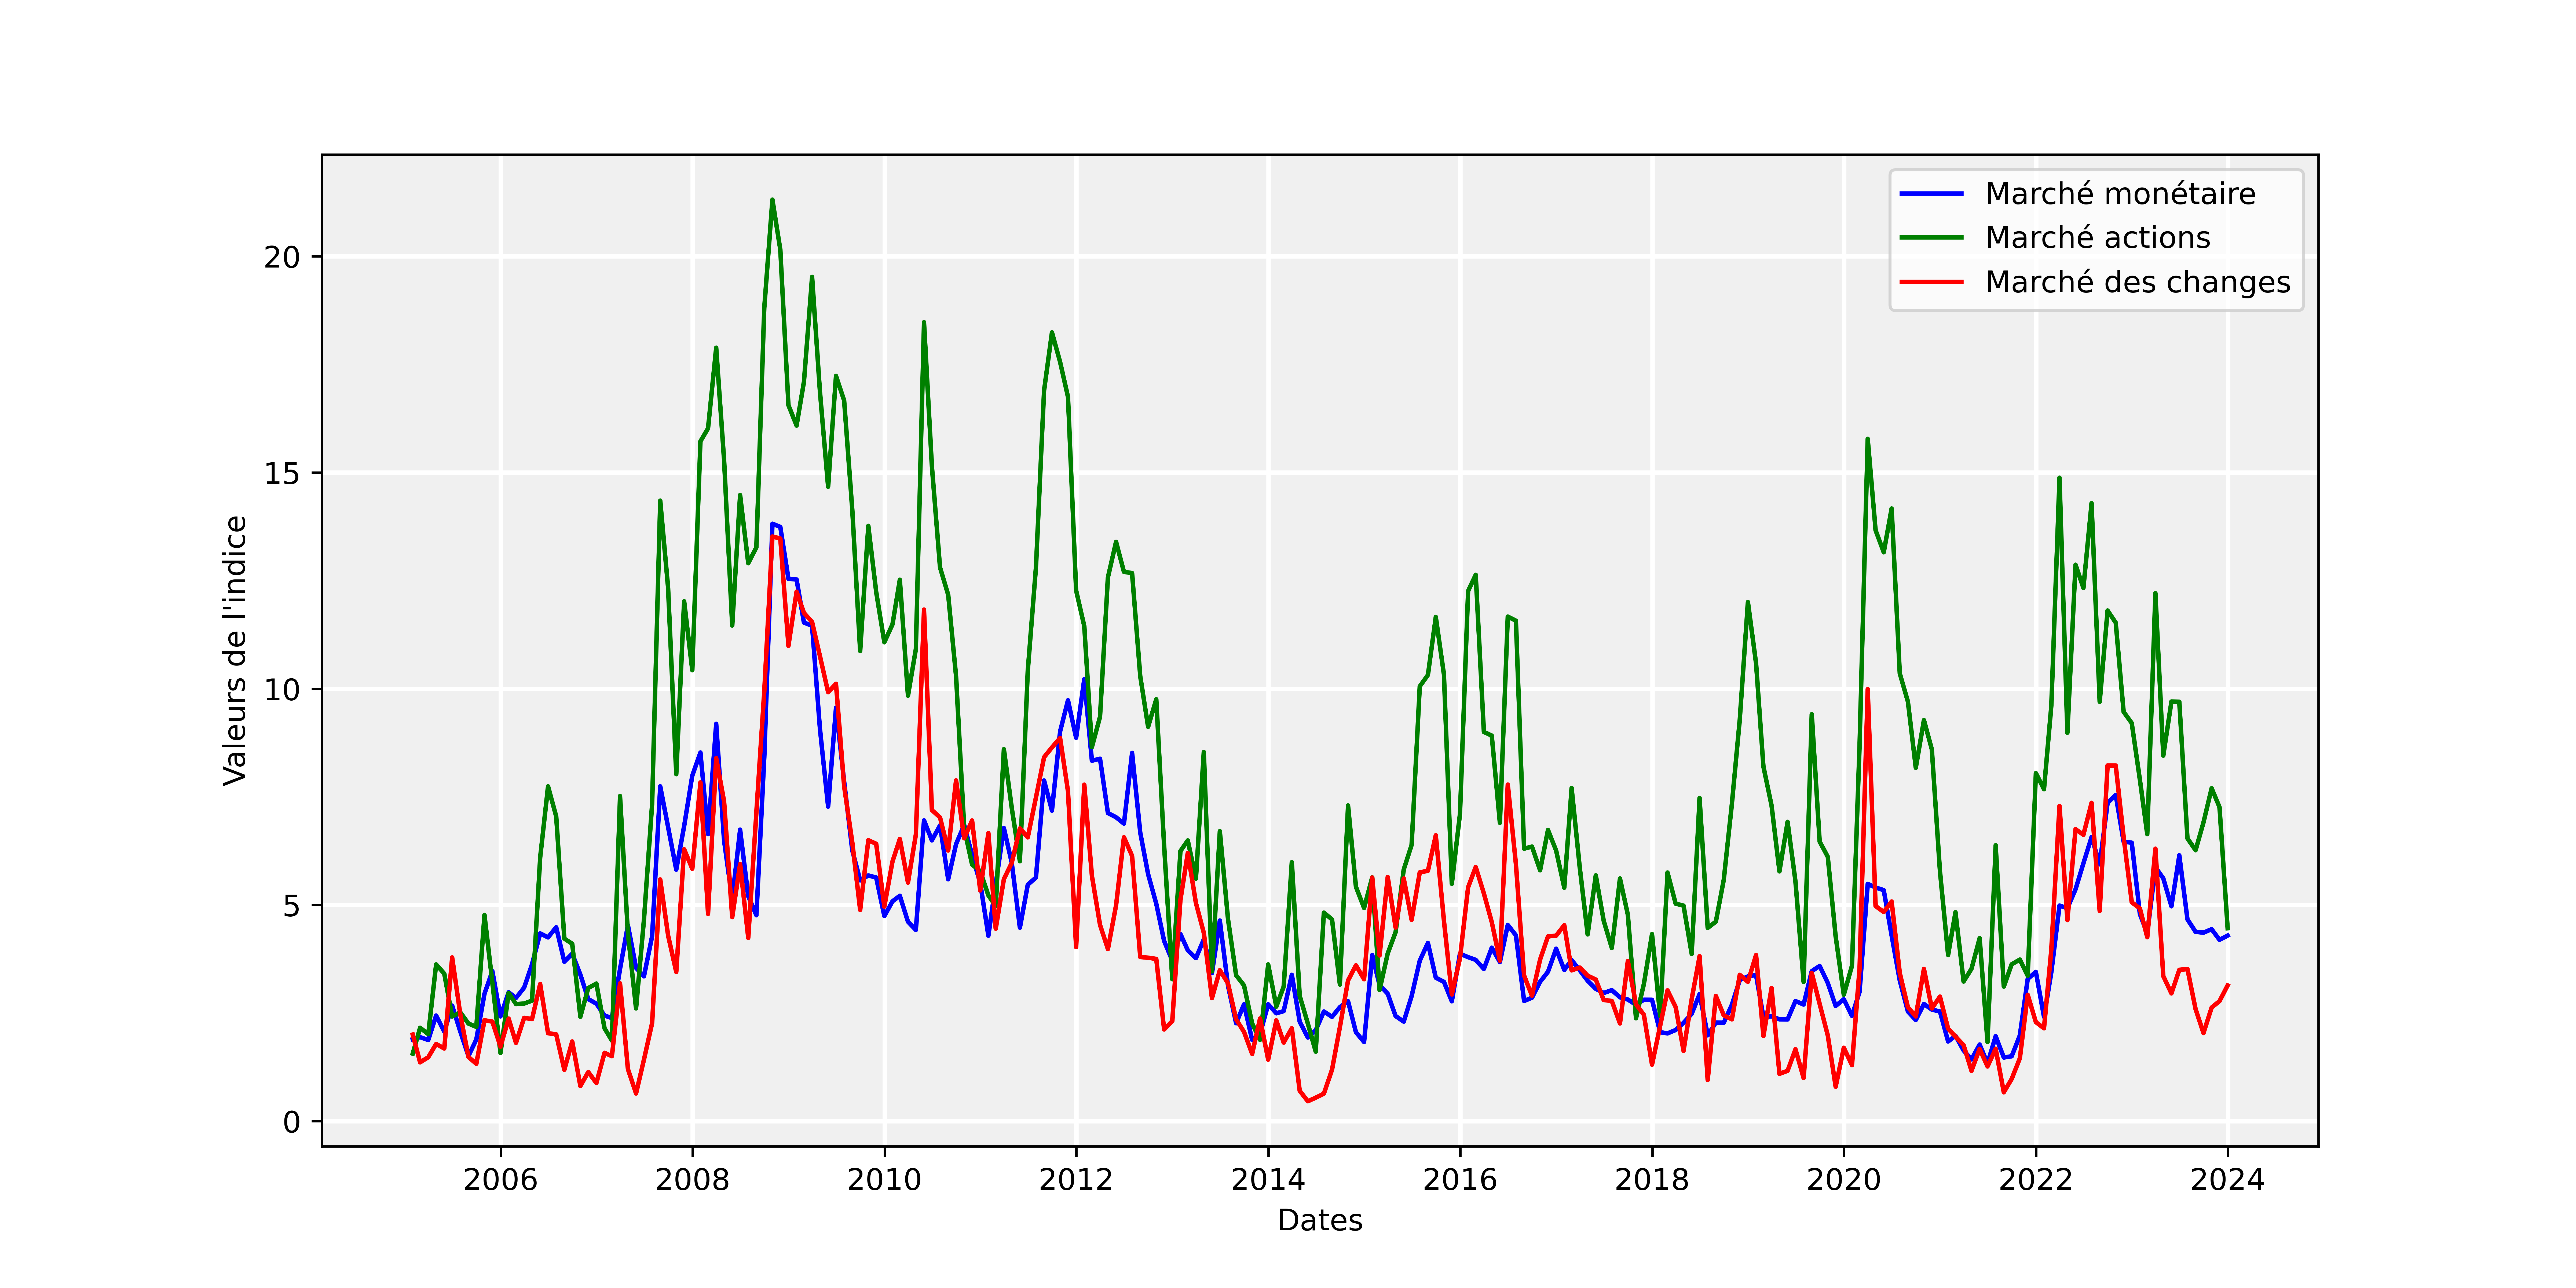
\includegraphics[width=1\linewidth]{figures/sous_indicateurs_stress.png}
    \caption{Sous-indicateurs de stress entre janvier 2005 et décembre 2024.}
    \label{fig:graphindicateurs}
\end{figure}

Le graphique montre l'évolution des sous-indicateurs de stress des trois principaux segments financiers (marché monétaire, marché des actions, et marché des changes) entre janvier 2005 et décembre 2024. Chaque indicateur est représenté par une courbe distincte : le marché monétaire est en bleu, le marché des actions en vert, et le marché des changes en rouge.\\

Le marché des actions montre la plus grande volatilité parmi les trois indicateurs. À plusieurs reprises, notamment entre 2008 et 2012 ainsi que vers 2020, on observe des pics marqués, correspondant à des périodes de forte tension sur ce marché. Le stress sur le marché des actions est particulièrement élevé lors des crises financières, comme celle de 2008, où le graphique montre une nette augmentation du stress. Après cette période de crise, le stress sur le marché des actions diminue progressivement, bien que des pics sporadiques apparaissent, notamment en 2020, ce qui pourrait être attribué à la crise liée à la pandémie de COVID-19. En général, la courbe verte représente des variations assez brusques, ce qui reflète la nature plus volatile du marché des actions, particulièrement sensible aux événements macroéconomiques et aux changements dans les conditions du marché mondial.

\begin{figure}[H]
    \centering
    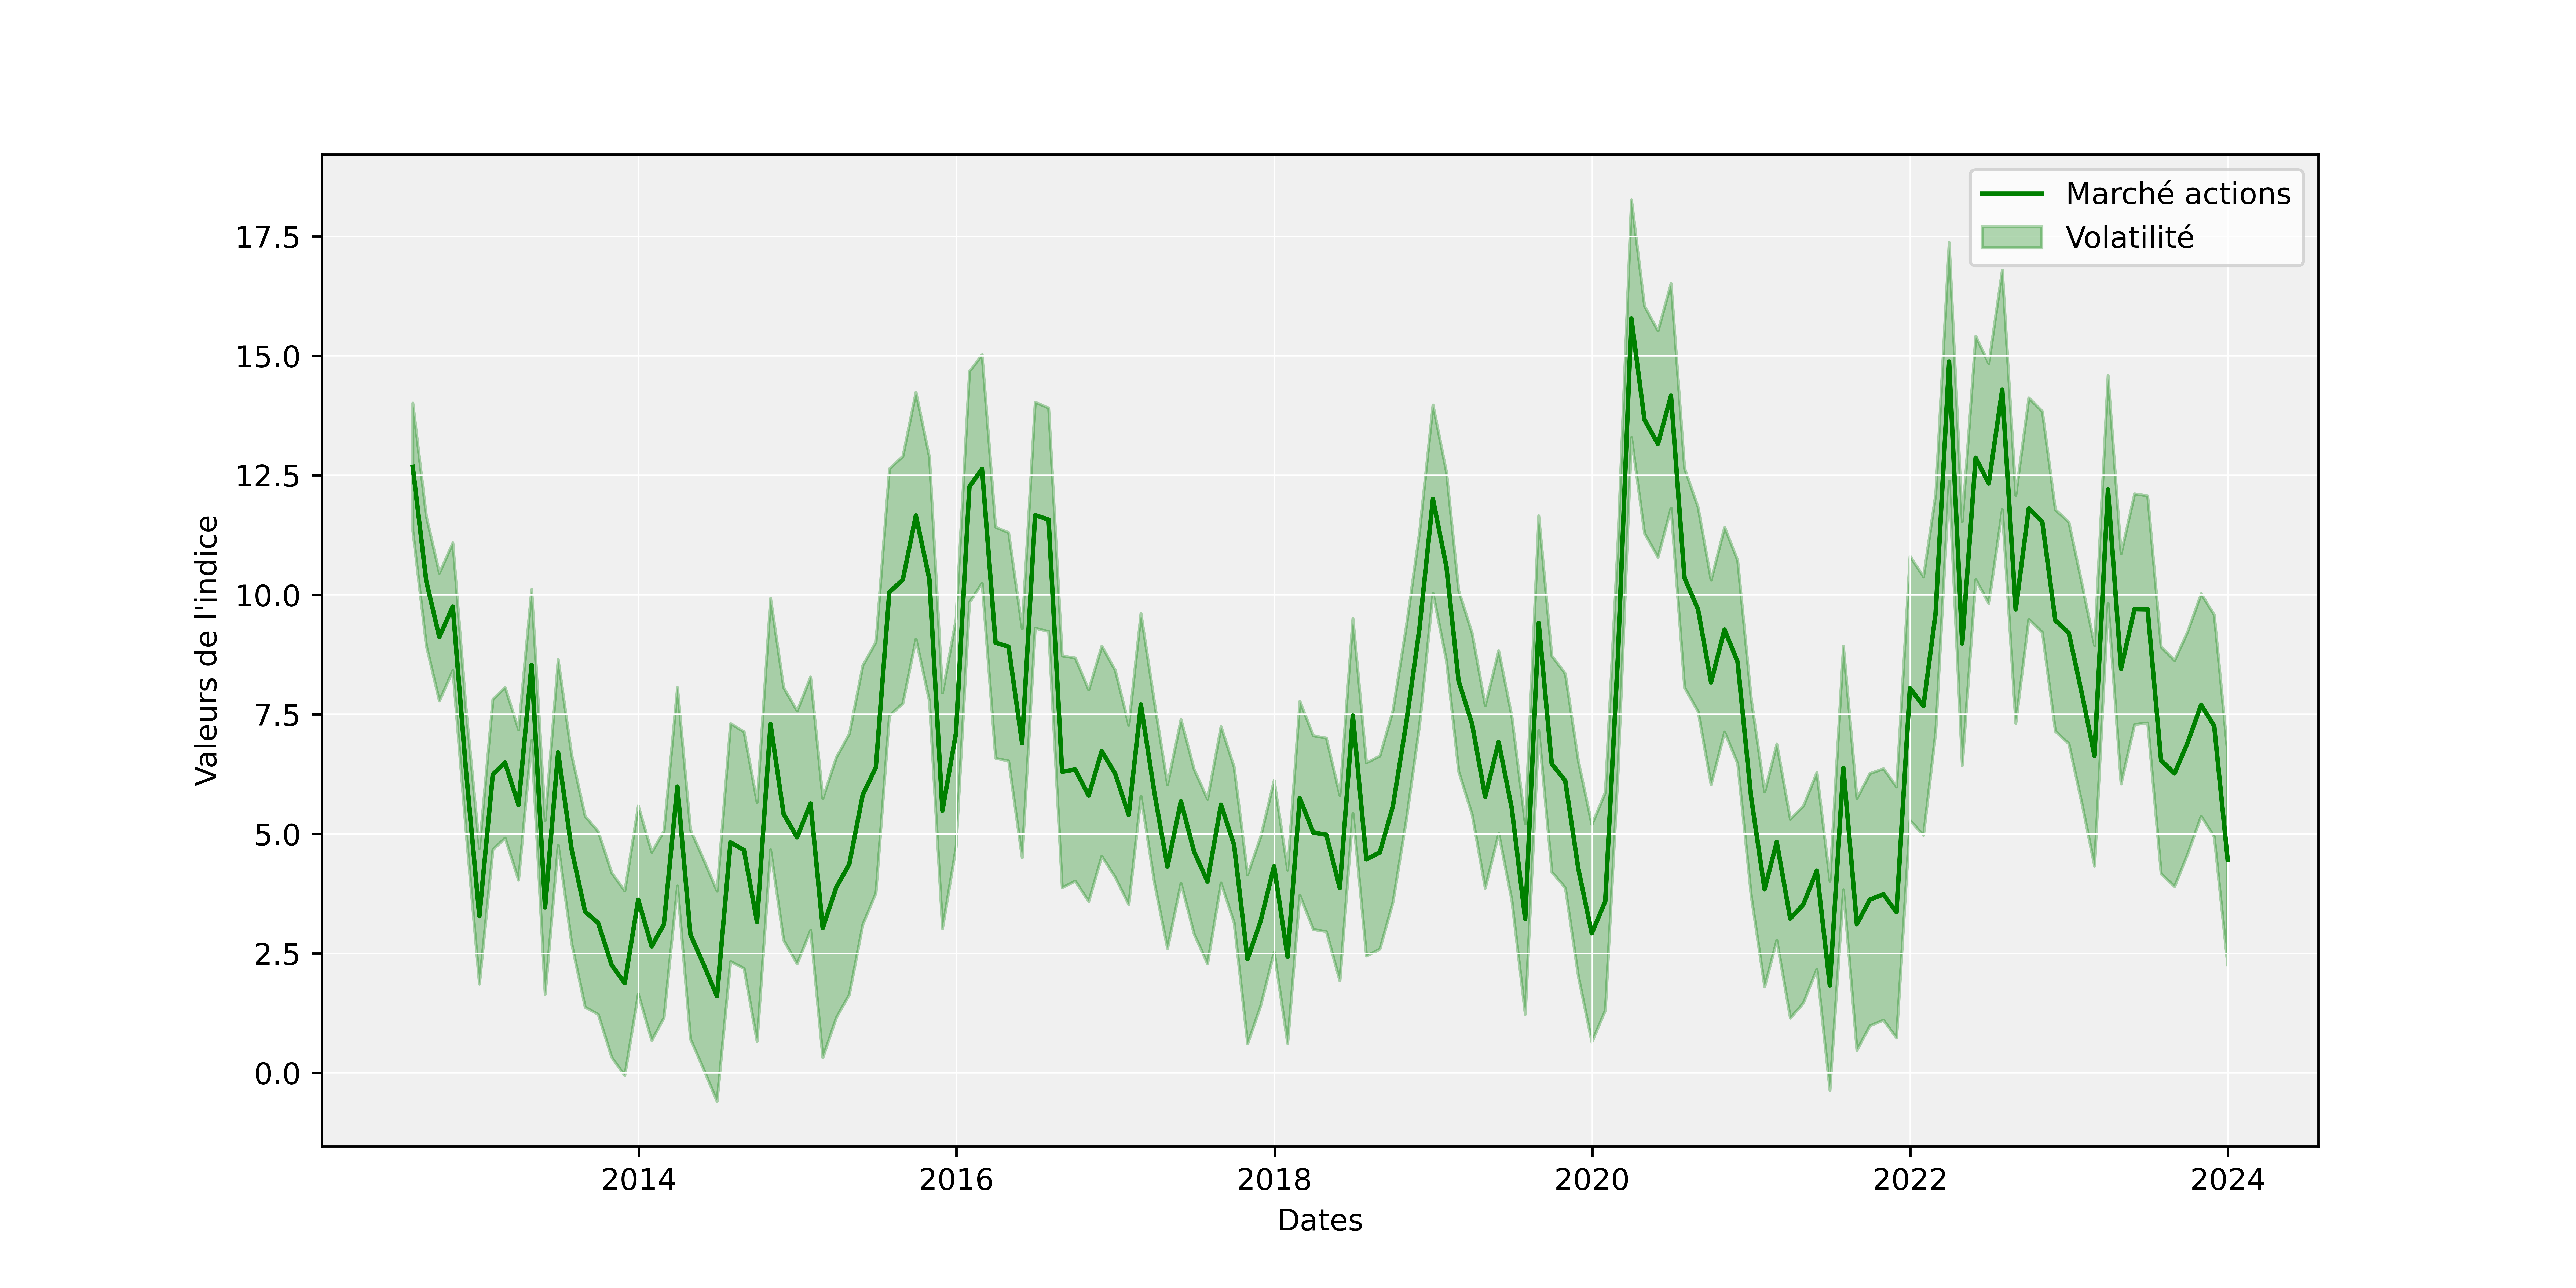
\includegraphics[width=1\linewidth]{figures/sous_indicateurs_equity_stress_equity.png}
    \caption{Stress sur le marché actions et volatilité associée entre janvier 2005 et décembre 2024.}
    \label{fig:enter-label}
\end{figure}

La volatilité observée sur le marché des actions suggère que les investisseurs réagissent fortement aux événements qui affectent la confiance dans les entreprises et l’économie en général. Les pics de volatilité élevés, particulièrement en 2008 et 2020, indiquent que les actions subissent des ajustements massifs des portefeuilles des investisseurs, souvent en raison de ventes paniquées ou de changements rapides dans les perspectives économiques.\\

En ce qui concerne le marché monétaire, cela montre des variations plus modérées par rapport aux autres marchés. Bien qu’il y ait des pics de stress, notamment autour des crises financières majeures, les valeurs de l'indicateur restent globalement plus stables. Cela reflète la nature plus régulée et contrôlée du marché monétaire, où les banques centrales interviennent régulièrement pour stabiliser les conditions de liquidité. Il est possible d'observer des pics importants autour de 2008 et un autre vers 2012, correspondant à la crise de la dette souveraine en Europe, ainsi que de légères hausses durant d'autres périodes de tension comme la crise de 2020. Cependant, contrairement au marché des actions, le marché monétaire retourne rapidement à des niveaux de stress plus bas après ces périodes de tension. Cela montre une capacité de stabilisation plus rapide dans ce segment du marché.

\begin{figure}[H]
    \centering
    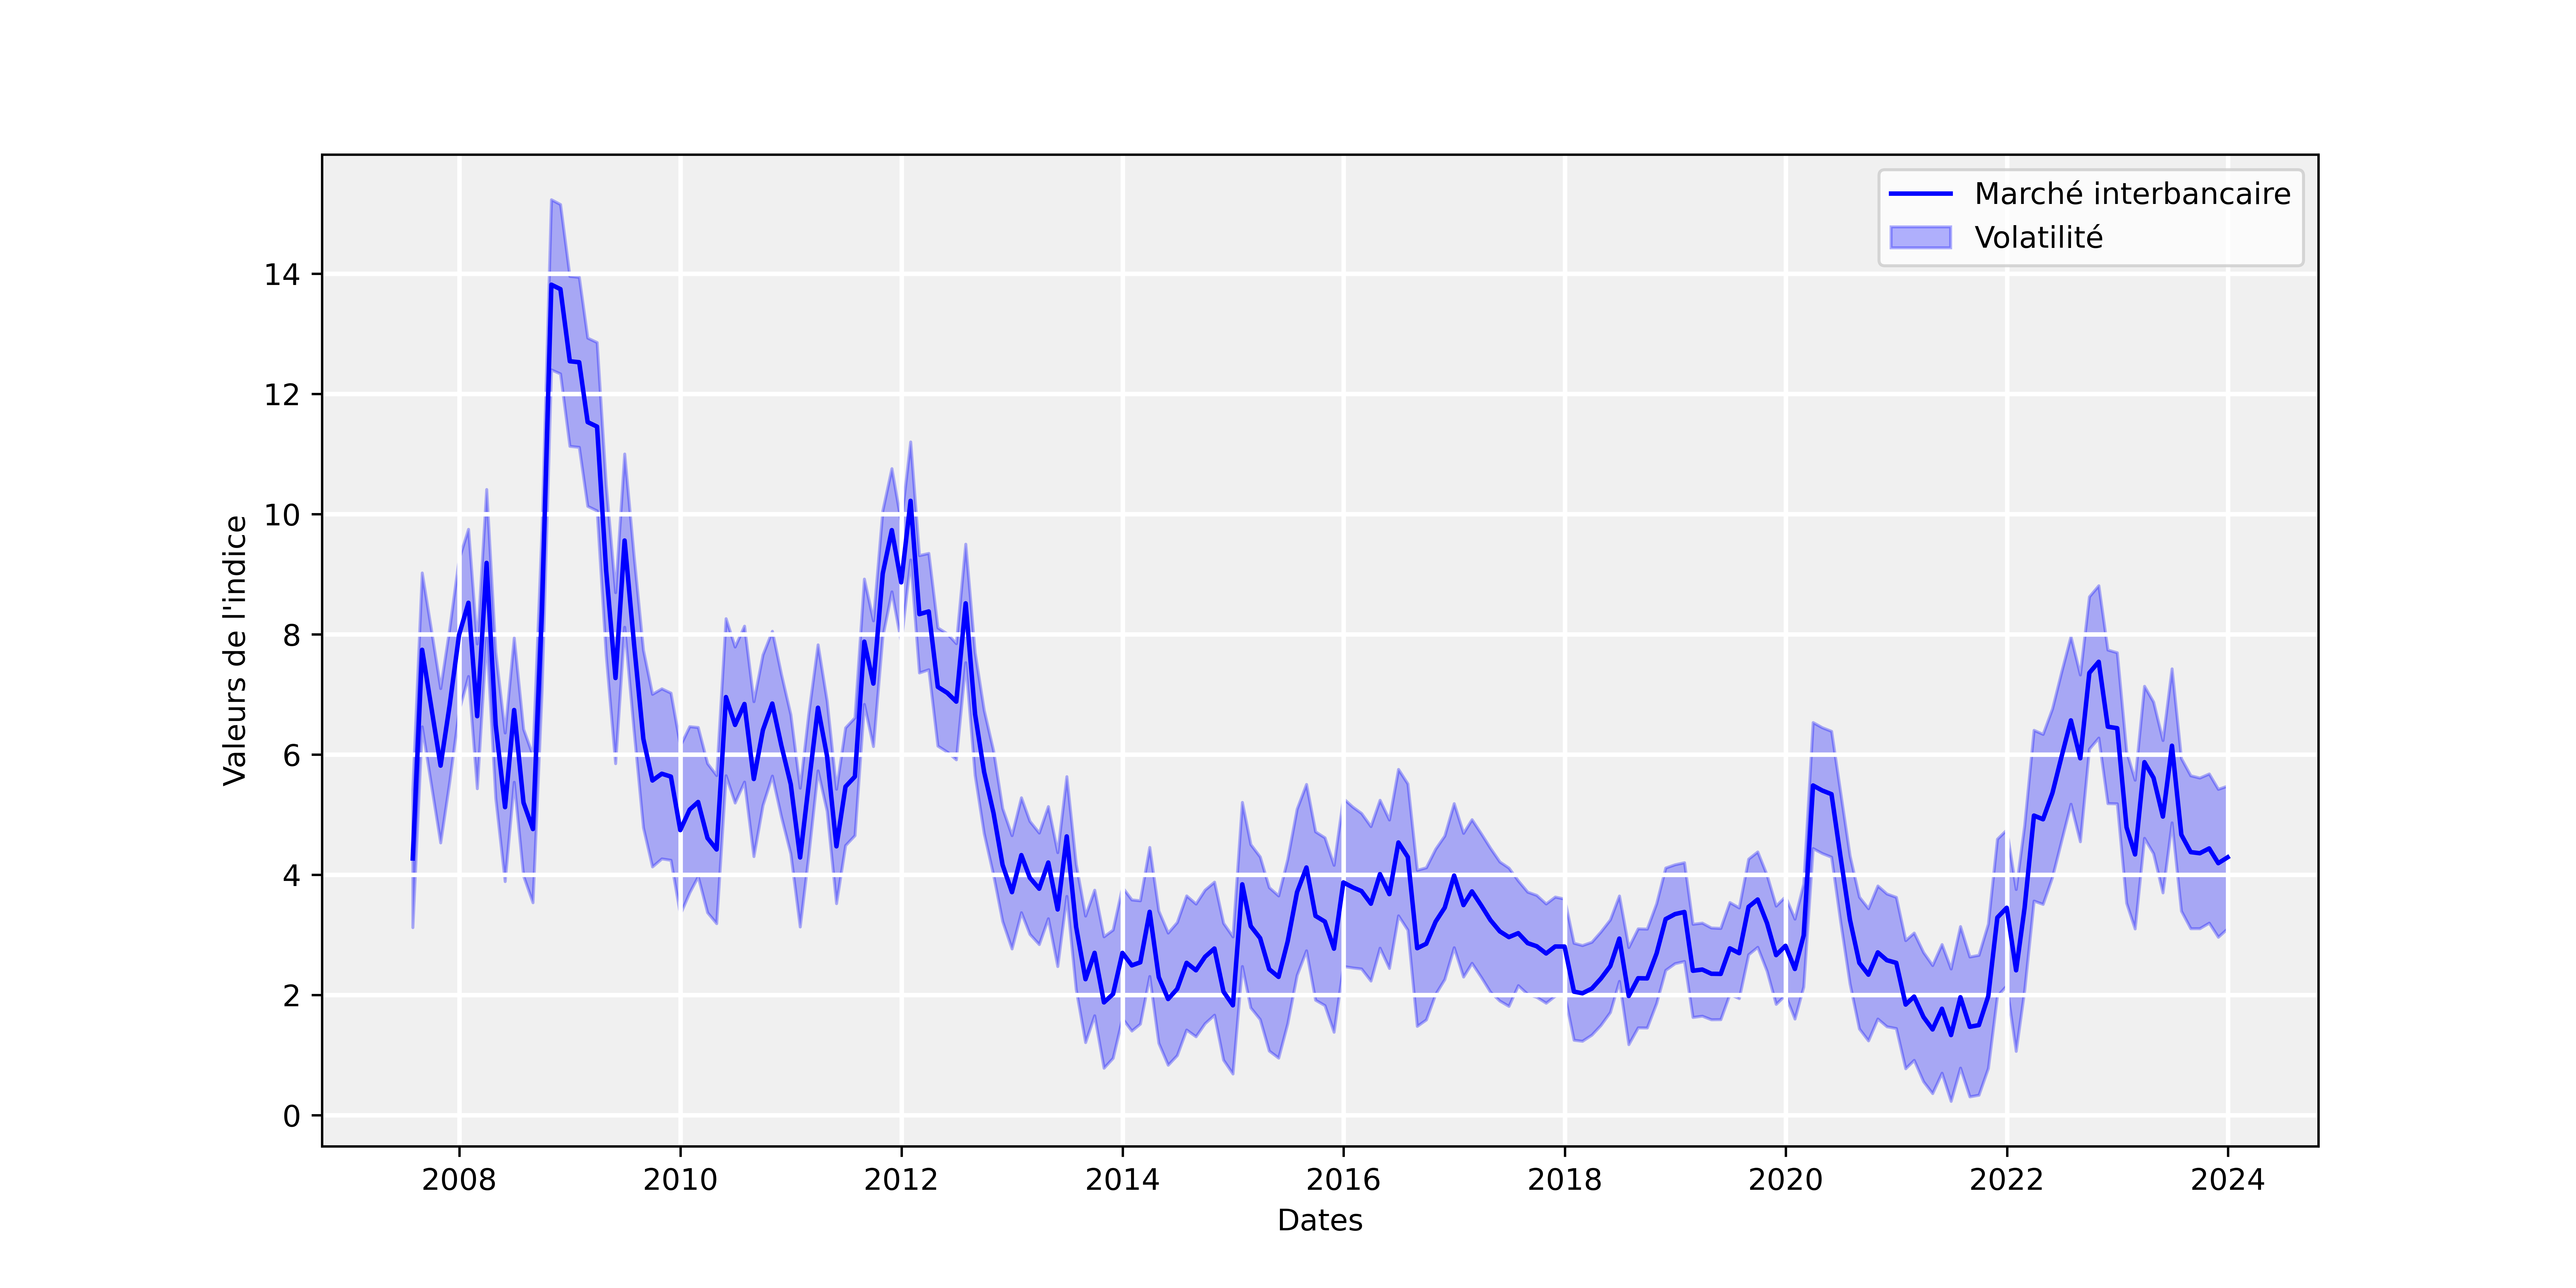
\includegraphics[width=1\linewidth]{figures/sous_indicateurs_stress_imm.png}
    \caption{Stress sur le marché monétaire et volatilité associée entre janvier 2005 et décembre 2024.}
    \label{fig:enter-label}
\end{figure}

La volatilité modérée associée au stress sur le marché monétaire, par rapport au marché des actions, est en partie due à la capacité des banques centrales à stabiliser ce marché via leurs outils de politique monétaire. Les pics de volatilité, en particulier en 2008 et 2011, sont le reflet des périodes où les banques hésitent à se prêter mutuellement, indiquant un risque accru de crise de liquidité. Cependant, après les interventions des régulateurs, la volatilité diminue rapidement, témoignant de la résilience de ce marché.\\

Enfin, le marché des changes est globalement le moins stressé parmi les trois segments, comme en témoignent les niveaux relativement bas de la courbe rouge. Cependant, ce marché montre également des épisodes de stress ponctuels, en particulier autour de 2008 et 2010-2012, ainsi que quelques augmentations notables dans les années plus récentes (vers 2020). La nature décentralisée et liquide du marché des changes lui permet de mieux absorber les chocs, bien que des périodes de forte volatilité, notamment causées par les fluctuations des taux de change et les crises monétaires, entraînent des pics soudains. Le stress sur ce marché semble être plus transitoire et moins soutenu que sur le marché des actions, où les tensions persistent souvent sur une plus longue période.

\begin{figure}[H]
    \centering
    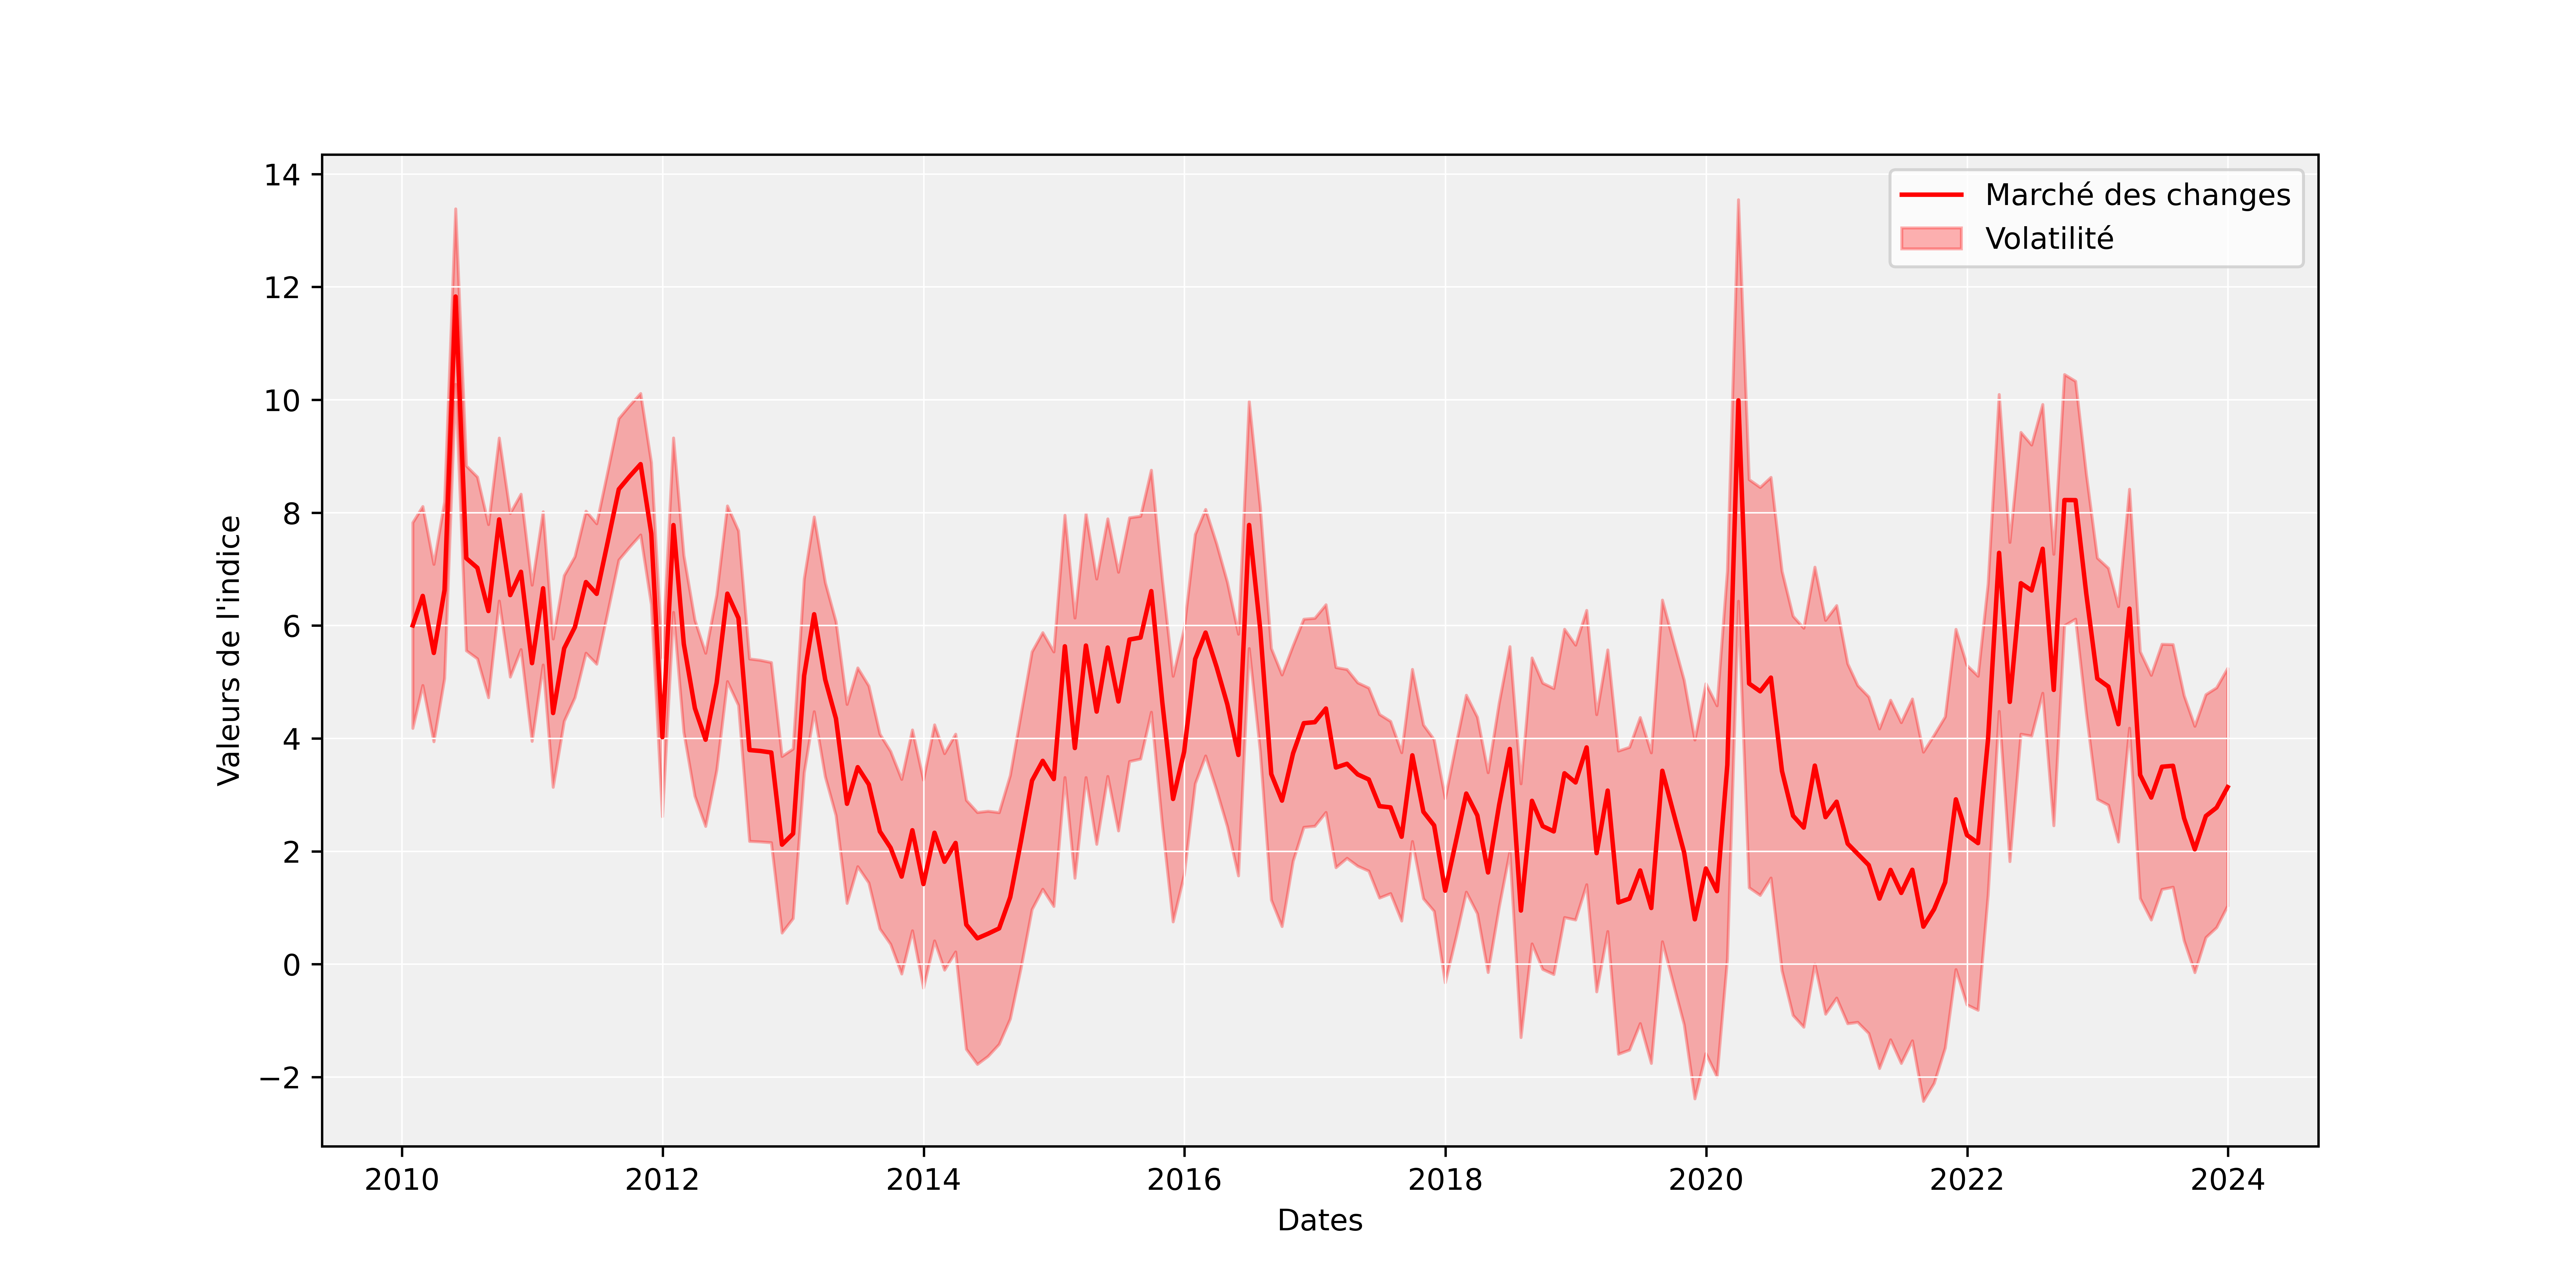
\includegraphics[width=1\linewidth]{figures/sous_indicateurs_forex_stress_forex.png}
    \caption{Stress sur le marché des changes et volatilité associée entre janvier 2005 et décembre 2024.}
    \label{fig:enter-label}
\end{figure}

La volatilité, qui accompagne les hausses de stress, est particulièrement importante autour de ces périodes. Les fluctuations observées en 2020 peuvent être attribuées aux mouvements des taux de change lors de la pandémie, ainsi qu'à la réponse des banques centrales à travers des ajustements des taux d'intérêt et des mesures non conventionnelles. Cependant, même si des périodes de stress apparaissent, le marché des changes tend à revenir à des niveaux de stress modérés sur le long terme, reflétant sa capacité à absorber les chocs grâce à sa liquidité élevée et à son caractère global.\\

En somme, l'interconnexion entre ces trois indicateurs de stress est bien visible. Lors des grandes crises financières, comme celle de 2008, on observe des pics simultanés dans les trois indicateurs, ce qui reflète un stress systémique à travers plusieurs segments financiers. Cependant, chaque marché semble réagir différemment en fonction de sa structure et de sa régulation. Le marché des actions tend à subir des chocs plus fréquents et plus sévères, tandis que le marché des changes montre une capacité à absorber les chocs avec des variations moins marquées. Le marché monétaire, quant à lui, présente une stabilité relative, malgré des tensions durant les périodes de crise.\\

Cette analyse démontre l'importance de surveiller l'évolution simultanée des sous-indicateurs de stress pour comprendre comment les tensions dans un segment peuvent se propager aux autres, exacerbant ainsi les crises financières. Après avoir effectué une analyse graphique des sous-indicateurs de stress pour les trois principaux segments financiers, l'analyse des statistiques descriptives va être mené. Cette approche permettra de mieux comprendre la distribution et les caractéristiques des différents indicateurs de stress en quantifiant leur tendance centrale, leur dispersion.

\begin{table}[H]
    \centering
    \sffamily
    \scalebox{0.9}{\begin{tabular}{lccccccc}
        \toprule
        \textbf{Indicateurs} & \textbf{Moyenne} & \textbf{Médiane} & \textbf{Maximum} & \textbf{Minimum} & \textbf{Écart-type} & \textbf{Skewness} & \textbf{Kurtosis} \\
        \midrule
        IMM      & 4.39  & 3.68  & 13.82  & 1.33  & 2.38  & 1.45  & 5.35  \\
        FOREX    & 4.19  & 3.52  & 13.52  & 0.46  & 2.65  & 1.09  & 4.07  \\
        EQUITY   & 8.02  & 6.91  & 21.31  & 1.56  & 4.56  & 0.68  & 2.64  \\
        \bottomrule
\end{tabular}


}
    \caption{Statistiques descriptives.}
    \label{fig:statsdescriptives}
\end{table}

L'analyse des moyennes montre que l'indicateur de stress sur le marché des actions  présente la valeur moyenne la plus élevée avec 8.02, suivie par les marchés interbancaire et des changes avec des moyennes respectives de 4.39 et 4.19. Cela suggère que, dans l'ensemble, le marché des actions tend à subir un stress plus important que les marchés des changes et interbancaire. En observant les valeurs médianes, il est possible de voir que le marché des actions affiche également la valeur médiane la plus élevée (6.91), ce qui renforce l'idée que ce marché est plus fréquemment sujet à des périodes de stress élevé. Les marchés interbancaire et des changes ont des valeurs médianes plus proches de leur moyenne, respectivement à 3.68 et 3.52, ce qui indique une distribution des données plus symétrique, bien que des périodes de stress aigu existent.\\

Les valeurs maximales et minimales montrent que marché des actions a connu des pics de stress beaucoup plus élevés, avec une valeur maximale de 21.31, contre 13.82 pour l'IMM et 13.52 pour le FOREX. De plus, les valeurs minimales montrent que le marché des changes a subi des périodes de stress très faibles avec une valeur minimale de 0.46, beaucoup plus basse que celles observées sur les marchés interbancaire (1.33) et des actions (1.56). Cela suggère que le marché des changes est potentiellement plus volatil avec des périodes de très faible stress ainsi que des pics de stress relativement élevés.\\

L'écart-type permet de mesurer la dispersion des données autour de la moyenne, il est aussi une mesure de la volatilité. L'indicateur de stress du marché des actions présente une dispersion plus large (4.56), indiquant une plus grande volatilité des niveaux de stress par rapport aux autres marchés. Le FOREX montre également une volatilité non négligeable avec un écart-type de 2.65, tandis que l'IMM affiche la plus faible volatilité avec 2.38.\\

En examinant les coefficients d'asymétrie, tous les indicateurs présentent une asymétrie positive, ce qui signifie que les périodes de stress extrême sont plus fréquentes du côté des valeurs élevées. Le marché interbancaire présente la plus forte asymétrie (1.45), ce qui indique que ce marché connaît des épisodes de stress élevé relativement rares mais intenses. Le FOREX est également assez asymétrique avec une valeur de 1.09, tandis que le marché des actions présente une asymétrie plus modérée avec un coefficient de 0.68. Enfin, les coefficients de kurtosis montrent des informations sur la forme de la distribution des stress. Le marché interbancaire présente une kurtosis de 5.35, ce qui indique une distribution leptokurtique, caractérisée par des extrêmes plus fréquents et des périodes de stress aigu prononcées. Le FOREX affiche également une kurtosis élevée à 4.07, tandis que le marché des actions présente une distribution plus aplatie (2.64), indiquant une distribution plus proche de la normale.\\

Cela montre donc que le marché des actions tend à subir un stress plus élevé et plus volatil que les marchés des changes et interbancaire. Cependant, les périodes de stress intense sur le marché interbancaire se caractérisent par des épisodes plus rares mais plus extrêmes, comme le montrent ses valeurs de skewness et de kurtosis.

\subsection{L'interconnexion et la contagion des sous-indicateurs étudiés}

Pour comprendre pleinement les interconnexions et les mécanismes de contagion entre le sous-indicateur de stress sur le marché des actions, des changes et le marché monétaire, il faut  reconnaître comment ces segments, qui forment des piliers du système financier, interagissent dans une dynamique systémique. La nature interdépendante de ces marchés signifie que des tensions dans l’un peuvent rapidement se propager aux autres, amplifiant ainsi le risque systémique. C’est précisément cette complexité et cette interdépendance qui justifient l’importance de construire des indicateurs de stress systémique comme le \textit{CISS}, afin de surveiller, anticiper et réagir aux crises qui pourraient perturber l’économie.\\

Premièrement, les interconnexions seront étudiées avant d'étudier les mécanismes de contagion afin de discuter dans un troisième temps les implications macroprudentielles et monétaires.\\

\subsubsection{Les interconnexions entre les trois sous-indicateurs}

Les sous-indicateurs de stress des marchés actions, des changes et monétaires sont fortement interconnectés. Cette interdépendance résulte de flux financiers partagés, de comportements synchronisés des investisseurs, et des politiques monétaires et fiscales qui affectent simultanément ces segments. En période de crise, ces interconnexions deviennent plus visibles, car les acteurs du marché ajustent rapidement leurs positions en fonction des tensions apparentes dans d'autres segments.\\

Tout d'abord, le sous-indicateur de stress sur le marché des actions reflète la volatilité et les pertes cumulées sur les principaux indices boursiers, notamment ceux des entreprises non financières. En période de stress, une volatilité accrue sur le marché des actions signale une incertitude grandissante quant à la rentabilité des entreprises, à la stabilité économique globale et au comportement des investisseurs. Ces derniers, lorsqu'ils perçoivent des risques élevés sur le marché des actions, peuvent chercher à réallouer leurs portefeuilles vers des actifs jugés plus sûrs, comme les obligations d'État ou les monnaies refuges. Ce phénomène de réallocation peut alors affecter d’autres segments financiers, créant un effet de contagion. Par exemple, une baisse généralisée des indices boursiers peut pousser les investisseurs à vendre des actions en masse, ce qui augmente la pression vendeuse sur le marché des changes lorsque ces ventes concernent des entreprises exposées aux fluctuations des devises.\\

Ensuite, le FOREX est un canal fondamental par lequel les politiques monétaires, les flux de capitaux et les événements macroéconomiques influencent directement les autres segments financiers. Le sous-indicateur de stress du FOREX capture la volatilité des taux de change et les tensions qui en découlent. En période de forte incertitude, une dépréciation rapide d'une devise, souvent provoquée par des déséquilibres économiques ou des ajustements des taux d’intérêt, peut entraîner une volatilité accrue sur ce marché. Cela affecte directement les entreprises multinationales, dont la rentabilité est liée aux variations des taux de change. Par conséquent, une volatilité sur le stress du marché des changes affecte la compétitivité internationale des entreprises cotées, provoquant une instabilité sur le stress du marché des actions. Cette interaction souligne l'importance des indicateurs composites, comme le CISS, qui permettent de surveiller simultanément plusieurs segments et d'évaluer l'impact global d'une crise dans l'un d'eux.\\

Enfin, le marché monétaire est essentiel pour garantir la liquidité à court terme et le financement des banques et autres intermédiaires financiers. Le sous-indicateur de stress sur ce marché suit la volatilité des taux interbancaires, les spreads entre les obligations d'État et les taux interbancaires, ainsi que le recours aux facilités de liquidité d'urgence fournies par les banques centrales. Une crise de liquidité dans ce segment provoque des effets immédiats sur les autres marchés, car les banques et autres institutions financières sont contraintes de liquider des actifs, y compris des actions et des devises, pour générer des liquidités. Cela aggrave les tensions sur les marchés des actions et des changes, en augmentant la pression vendeuse et, par conséquent, la volatilité sur l'ensemble du système financier. La surveillance du marché monétaire est donc primordiale pour détecter et prévenir les crises de liquidité pouvant rapidement se propager à d'autres segments.

\subsubsection{Mécanismes de contagion entre les trois sous-indicateurs}

Les interconnexions observées entre ces trois sous-indicateurs de stress sont renforcées par des mécanismes de contagion, qui rendent les marchés particulièrement vulnérables aux chocs extérieurs. Ces mécanismes s'intensifient surtout en période de crise, lorsque le stress dans un segment localisé s'étend rapidement aux autres, créant un effet domino.\\

Un première peut être que le marché monétaire est un canal principal de transmission des chocs financiers, car il assure la liquidité nécessaire au bon fonctionnement des institutions financières. En période de crise, lorsque les taux interbancaires augmentent de manière significative, les institutions financières se retrouvent en situation de tension de liquidité. Pour compenser, elles vendent des actifs, notamment des actions et des devises, amplifiant ainsi la volatilité sur ces marchés. Ce cercle vicieux où la vente massive d’actions exacerbe la baisse des cours, alimente les incertitudes et accroît les tensions sur les autres marchés, démontre l’importance d’un suivi étroit des tensions de liquidité. Le stress monétaire peut également affecter le marché des changes, car les banques rapatrient des capitaux ou ajustent leurs positions en devises pour faire face à leurs besoins de liquidité, amplifiant la volatilité sur le FOREX.\\

Il est possible d'évoquer les stratégies d'arbitrage, qui consistent à exploiter les différences de prix entre les actifs, constituent un autre mécanisme de contagion important. Lorsqu'une volatilité significative apparaît sur le marché des actions, les investisseurs ajustent souvent leurs positions sur le marché des changes pour couvrir les risques de change, ou pour spéculer sur les variations futures des devises. Cela entraîne une volatilité accrue sur le FOREX, aggravant les tensions dans ce segment. Par ailleurs, lorsque les investisseurs cherchent à limiter leurs pertes sur un marché, ils réallouent leurs portefeuilles vers d'autres marchés plus stables, ce qui exerce une pression supplémentaire sur l'ensemble du système financier.\\

Aussi, lors des périodes de crises financières, les investisseurs tentent généralement de protéger leur capital en transférant leurs fonds vers des actifs jugés plus sûrs, tels que les obligations d'État ou les devises stables, comme le dollar américain. Ce mouvement, appelé "fuite vers la qualité", affecte directement le marché des changes, car les devises refuges connaissent une hausse de la demande, entraînant des fluctuations importantes des taux de change. Ce phénomène a des répercussions sur les marchés actions, en particulier pour les entreprises exportatrices, dont les revenus dépendent des variations de change. En effet, une forte appréciation des devises refuges peut rendre les exportations plus coûteuses, réduisant ainsi la compétitivité des entreprises sur les marchés internationaux et aggravant les tensions sur les marchés actions.

\subsubsection{Rôle des politiques monétaires et macroprudentielles}

L’un des principaux objectifs de la BCE et des régulateurs financiers est de maintenir la stabilité financière tout en garantissant une inflation maîtrisée. Dans ce contexte, les sous-indicateurs de stress des marchés des actions, des changes et monétaires, ainsi que le CISS, jouent un rôle clé dans la surveillance du système financier et dans l'orientation des politiques monétaires et macroprudentielles. Ces indicateurs fournissent des signaux précoces qui permettent d’ajuster les politiques en fonction des tensions observées sur les différents marchés.\\

L'intérêt de construire des indicateurs comme le CISS réside dans leur capacité à capturer les interconnexions entre les différents segments financiers et à identifier les périodes où le stress est suffisamment élevé pour entraîner une contagion systémique. Le CISS offre une vision d’ensemble des risques systémiques en agrégant les sous-indicateurs des marchés actions, des changes et monétaires, tout en tenant compte de leurs corrélations dynamiques. Cela permet aux décideurs politiques de mieux anticiper les crises et d'intervenir de manière préventive pour éviter une amplification des tensions.\\

Par exemple, en surveillant l'évolution du CISS, la BCE peut évaluer à quel moment les tensions sur un segment donné, comme le marché monétaire, deviennent suffisamment importantes pour justifier une intervention. Cela pourrait inclure des injections de liquidités sur le marché monétaire ou un assouplissement des taux d'intérêt pour soutenir les banques en période de tension. De plus, en ajustant les exigences de fonds propres des banques ou en mettant en place des coussins de capital anticrises, la BCE peut renforcer la résilience du système bancaire et réduire la contagion potentielle des crises. Ainsi, l’analyse des indicateurs de stress systémique permet non seulement d'identifier les moments critiques où une intervention est nécessaire, mais aussi d'adapter les outils macroprudentiels pour prévenir des crises futures.\\

L’étude des interactions entre les différents segments du système financier, ainsi que l’élaboration d’indicateurs comme le CISS, mettent en évidence la complexité et l’interdépendance des marchés financiers modernes. À travers une analyse approfondie des marchés des actions, des changes et monétaires, cette partie a montré comment les tensions systémiques se développent et se propagent, illustrant ainsi la nécessité d’une surveillance holistique et proactive. L’approche intégrée du CISS, qui combine des indicateurs spécifiques avec des corrélations dynamiques, représente un outil clé pour évaluer les risques systémiques et guider les politiques monétaires et macroprudentielles.\\

Les mécanismes de contagion, tels que la propagation via la liquidité ou les ajustements de portefeuilles, soulignent l’importance de comprendre les interactions entre segments pour anticiper les crises systémiques. En outre, l’analyse des sous-indicateurs a révélé que chaque marché, bien que distinct dans sa structure et ses dynamiques, contribue de manière significative à l’évaluation globale du stress financier. Les marchés des actions se caractérisent par leur volatilité accrue, les marchés des changes par leur résilience, et les marchés monétaires par leur rôle critique dans la fourniture de liquidités, illustrant ainsi la complémentarité des segments.\\

Cette partie a également mis en lumière l’utilité pratique du CISS pour les régulateurs et les décideurs politiques, en leur fournissant des outils pour surveiller et stabiliser le système financier. En anticipant les périodes de stress systémique et en ajustant les politiques en conséquence, les autorités peuvent limiter l’impact des crises financières sur l’économie réelle, protégeant ainsi la croissance économique et la stabilité sociale.\\

Après avoir établi les fondements théoriques et méthodologiques du CISS, l’analyse se tourne désormais vers la méthodologie économétrique utlisée dans ce projet. Cette transition est nécessaire pour quantifier les relations dynamiques entre les sous-indicateurs de stress, mesurer les interactions entre les marchés et évaluer empiriquement les mécanismes de contagion identifiés. La partie économétrique s’appuiera sur des modèles non-linéaires adaptés, notamment des modèles MS-VAR et NARDL.

\end{sloppypar}

